\epigraph{\textit{The business changes. The technology changes. The team changes. The team members change. The problem isn't change, per se, because change is going to happen; the problem, rather, is the inability to cope with change when it comes.}}{-- \textup{Kent Beck}}

During the early stages of the development, the first steps we followed were highly related to polishing and improving the solution described in the previous chapter. This was a challenging problem that resulted in a change in the project's direction, which will be detailed later.

\section{Technology stack}

As I mentioned earlier, the purpose of this second solution was to improve what was already implemented. This way, we kept most of the stack untouched. The sole change was the replacement of GraphX with its DataFrame equivalent library named GraphFrames.

\begin{figure}[ht]
    \centering
    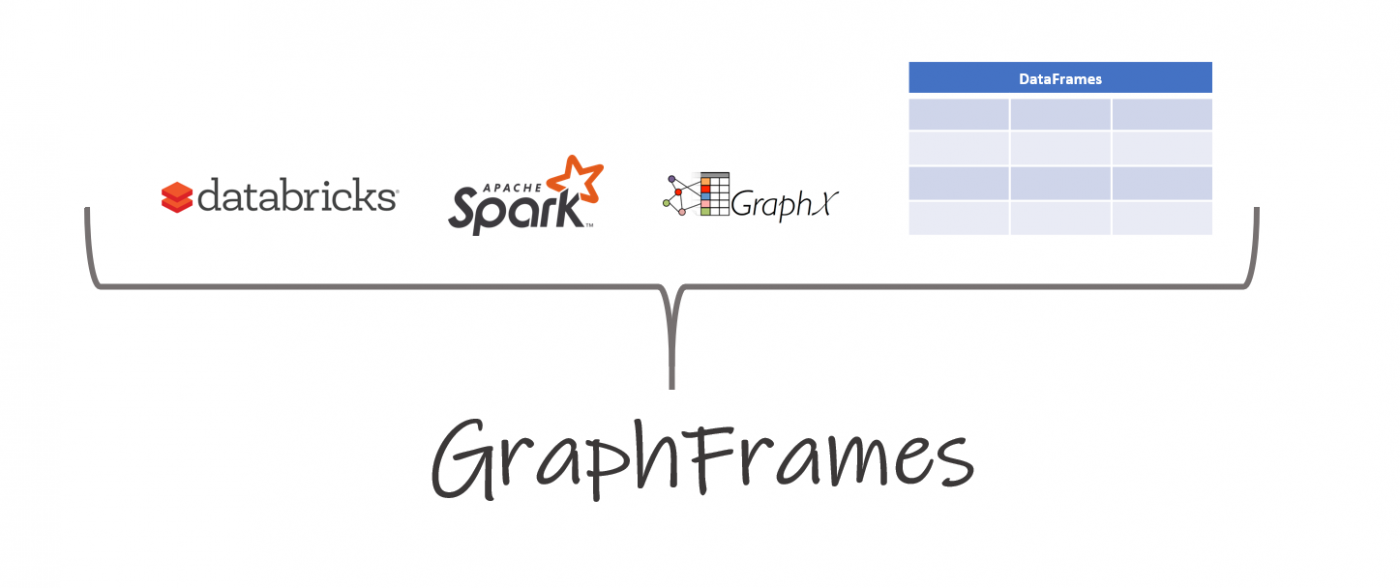
\includegraphics[width=.7\linewidth]{img/8-1_graphframes.png}
    \caption[Stack of the different technologies we are using for the second solution]{Stack of the different technologies we are using for the second solution\footnotemark}
\end{figure}

\footnotetext{\url{https://adatis.co.uk/graphframes/}}

\subsection{GraphFrames}

As it name goes, GraphFrame is a package for Apache Spark providing support for DataFrame-based Graphs. According to the introductory lines, the main goal of this stage of the development was to move our solution one step further in the abstraction level, from a solution based on RDDs to another based on DataFrames. From the ground up, we always believed RDDs weren't the go-to. What's more, RDDs are discouraged as they seem to be outdated in comparison to DataFrames and Datasets. More into this will be discussed in the next section.

\subsection{DataFrames and Datasets}

From Spark version 1.3 onwards, what were once known as SchemaRDDs are now referred to as DataFrames. That may give us an idea of what a DataFrame is. In that sense, they basically are RDDs provided some Schema for the data that is collected. With the help of this schema, DataFrames may be seen as rows with uniform structure: columns. Whereas RDDs are more akin to objects, DataFrames are closer to a table in a data base. This is quite relevant, as managing schemas to describe data allows us to perform operations over data in a much more efficient way than using Java serialization. It is worth mentioning that from Spark version 2, DataFrames can be understood as a type alias for \texttt{Dataset[Row]}, as they merged both APIs. In that sense, Datasets can be seen as the combination of the best from both worlds: with the appearance of a Java object from the outside, but with the shape of a table in RDBMS internally.

We now have a clear vision of what a DataFrame is. The problem is that even though they provide some nice features for data wrangling: schemas allow us to establish contracts so consumers know exactly the shape of the data they are working with, they are not so nicely implemented currently. Not only Apache Spark has no official support for working with DataFrame-based Graphs: notice GraphFrames is required, but the variety of supported types is scarce: including primitive types and Dates. Long has been discussed in this sense, but nothing has really changed since 2015\footnote{\url{https://issues.apache.org/jira/browse/SPARK-7768}}. To clarify this, let's put it into perspective.

\subsubsection{Encoders and User-defined Types}

Working with simple data-structures is a trivial task in Apache Spark. What is not so easy to handle are custom data types. If the DataFrame cannot implicitly retrieve an Encoder, the user will be informed to provide one. This is needed for Spark SQL to infer the schemas of the data we are working with. The complex the data-structure, the harder it is for the programmer to write an appropriate serialization/deserialization mechanism. Other solution could be writing your own User-defined types, which can be understood as wrappers for the actual types. However, the amount of boiler-plate code and complexity of the data to be stored makes this a tedious process. Lastly, notice how this solution is far from efficient as it is also based on serialization for data storage and retrieval.

\subsubsection{The Catalyst Optimizer}

\section{Implementation of the Second Pregel solution}